\chapter*{LOS VIDEOJUEGOS EN LINUX}

\section*{INTRODUCCIÓN}
En la sociedad surgen muchas necesidades, sea por razones
personales o laborales, a consecuencia de ello se tratan de
solucionar de una forma más eficaz, en un mundo laboral difícil
de llevar genera mucho estrés, para los amantes de los
videojuegos este tema les va a parecer muy interesante el tema
del desarrollo de los videojuegos sobre y para el sistema
operativo Linux, lo cual abarca muchos opciones a tratar por
ejemplo: los pasos, requerimientos y la tecnología necesaria
para la creación, mejorar y gestionar el desarrollo de un nuevo
video juego. Para esto hay que comprender que hay muchos
tipos de software libre o código abierto, juegos comerciales o los
que son portados a Linux, como también se comprende que hay
consolas para correr los videojuegos como lo es Pandora o
SuperGamer.

Con el avance de la tecnología, han surgido nuevas plataformas,
para esta ocasión es muy importante mencionar a Android, la
cual esta tiene un núcleo basado en kernel Linux, pero hay que
dejar claro que no tiene que ver absolutamente nada con el
mercado de juegos de Android, también ha tenido muchas
relaciones con otras plataformas, como el de MAC.

Lastimosamente el mercado de juegos para pc en sistemas
operativos distintos a Windows, actualmente es muy reducido,
ya que la mayoría de las empresas desarrolladoras que tienen un
alto título en desarrollos comerciales más importantes del
mundo, solamente desarrollan sobre Windows por su fácil
manejo y de algún modo lo ven como reducción de costos.
Pero también se pueden resaltar muchos puntos buenos en el
desarrollo de videojuegos en el sector económico y que de
muchas formas ha levantado este sector a base de tecnología
interactiva. Muchos críticos empresariales han tomado este
nuevo impacto y usarlo como una herramienta para el
desarrollo de la sociedad, de esta forma se plantea y se
desarrolla aplicaciones para el sector de la educación, promover
simulaciones empresariales, así muchas personas que tienen
mucho interés en los videojuegos, no solo para programadores si
no personas que desean obtener un conocimiento previo para
llegar al punto de realizar uno de ellos, verán herramientas que
tendrán la posibilidad de crear juegos complejos sin utilizar ni
una sola línea de código.

\section*{RELATOS SOBRE VIDEOJUEGOS YA EXISTENTES}
 
Como lo han planteado muchos contribuyentes y amantes al
desarrollo del software libre, Linux ha llegado a tener un gran
impacto en muchas ramas de la tecnología, es este relato se
habla en la parte de desarrollo de videojuegos, el sistema
operativo Linux hace parte de una listas más importantes de
software libre para gestionar un proyecto interactivo y por
aquello tiene muchas aplicaciones y modo de uso en la sociedad
que trabajan en el desarrollo de la tecnología. Aunque han
llegado a la conclusión que Linux no ha sacado al mercado
muchos videojuegos por ciertas razones, las que más se resaltan
es la del no conocer las capacidades del sistema operativo
correspondiente al desarrollo de nuevos software sea para el
campo laboral como para el campo interactivo, el otro factor
importante para nombrar es el gran auge que empezó hace unos
poco años sobre el desarrollo de videojuegos de alta gama, es
decir: Excelentes gráficos, buenos soportes, muy similares a la vida real y sobre todo ilustrativos.

Linux en los últimos años, se ha dedicado mucho a la creación
de videojuegos con la capacidad de tener una plataforma en la
red, más conocidos como los juegos de rol en primera persona
Online. Al momento de aparecer esta nueva forma de gestionar,
desarrollar y plantear un videojuego de este tipo, Linux ha
sacado al mercado muchos de ellos para consolas por medio de
Steam. Para lo que no saben que es Steam: es una plataforma de
distribución digital, gestión digital de derechos, comunicación y
servicios multijugador que fue desarrollada por la empresa Valve
Corporation. Es utilizado por pequeños desarrolladores
independientes como también lo usan grandes empresas y
corporaciones de software para la distribución de videojuegos y
material multimedia relacionado en este campo.

Los videos juegos ya existentes, en la actualidad a pesar de
tener un gran tiempo de ser desarrollados, por su gran auge,
comentarios y excelentes puntos de vista de los gamers han
estado en la lista de poder ser actualizados, sacar una segunda e
incluso tercera parte, entre muchos otros factores.

Unas de las ventajas más importantes e impactantes que tiene
Linux respecto a los videojuegos es que mientas estos en
Windows pueden llegar a costar decenas e incluso cientos de
dólares para poder adquirirlo, en Linux sencillamente son gratis,
bajo ninguna circunstancias o requerimientos, el único requisito
primordial es que sean ejecutados en este mismo sistema
operativo, pero aun así la gran cantidad de videojuegos
desarrollados para Windows pueden llegar a tener más impacto,
lo que lleva a que la comunidad gamers que solo se dedica al uso
de Linux les pueda parecer más atractivo lo que crea Windows y
migre a su uso.

\section*{IMPACTO EN LA SOCIEDAD}

Una de las razones por las cuales la gente normalmente no usa
Linux es por sus limitaciones a nivel de videojuegos, sí, esta es
una de las razones por las que los usuarios no se cambian
definitivamente a Linux y deciden conservar una partición con
Windows para su diversión y entretenimiento, pero al paso de
los años se han visto grandes avances en este aspecto, existen
videojuegos como Lugaru ó Neverwinter Nights que para suerte
de los amantes a los videojuegos de rol en línea fue parchado
para el sistema operativo del famoso pingüino, tuvo un muy
buen recibimiento por parte de los usuarios ya que dicho parche
crea una especie de instalación nativa para Linux y genera un
buen funcionamiento a la hora de jugarlo. Pero también
podemos hablar de cómo jugar videojuegos comerciales en
Linux y quitar esa barrera que separa el uso de Windows para
los videojuegos que tanto nos llaman la atención, nos referimos
a opciones como WINE y PLAY ON LINUX.

WINE es una re implementación de la interfaz de programación
de aplicaciones de Win16 y Win32 para sistemas operativos
basados en Unix, no podríamos decir que es un simple emulador
de Windows para Linux, es mejor referirnos como “Una
aplicación creada por ingeniería inversa” que nos permite tener
una especie de mini sistema Windows en nuestro Linux y que
podamos aprovecharlo no solo para los videojuegos, sino para
muchas aplicaciones de este SO que lleguemos a necesitar.
WINE es una herramienta a la que le podemos sacar mucho
provecho pero si queremos enfocarnos sólo en los videojuegos
podemos ver más hacia PLAY ON LINUX, esta es una aplicación
cuya base es WINE pero enfocada principalmente en ejecutar
videojuegos de sistemas Windows en ambiente UNIX y
GNU/LINUX, lo más interesante de esta aplicación es que
basada en problemas que llega a generar WINE en la instalación
de videojuegos, problemas que llegan a disminuir el rendimiento
de la aplicación, fue creada para configurar a su aplicación
madre para la adecuada ejecución de los videojuegos mediante
scripts que modifican su comportamiento y así ofrecer una mejor
ejecución, estos scripts también pueden ser creados por los
usuarios y adicionarlos para arreglar bugs, su extensión de
archivo es “.pol”.

Ya que hemos hablado de cómo aun en nuestro sistema
operativo basado en Linux podemos seguir jugando y
frecuentando nuestros videojuegos favoritos, pero veamos más
allá, en la raíz de todo, el desarrollo de estos. La pregunta es
¿Por qué grandes desarrolladores no diseñan videojuegos para
Linux?... Con respecto a esta pregunta que tantos se hacen y
muy pocos se atreven a responder se pueden plantear dos
aspectos.

Aspectos técnicos: Quizá una de las razones por las cuales
grandes desarrolladores y empresas que se dedican a la
producción de videojuegos de gran impacto como EA, Bizzard y
más, es que los controladores libres para las tarjetas gráficas
no son competentes para videojuegos, podrá verse como una
declaración un poco absurda pero tiene algo de razón, ya que los
fabricantes de tarjetas gráficas no han llegado a liberar
totalmente sus códigos para que usuarios creen controladores
competentes y libres. También podemos referirnos a un punto
muy discutido en la Web es que hay librerías que no son
compatibles con Linux por problemas de licencia o porque no
están portadas, pero también es un punto refutable ya que casi
que cualquier cosa puede ser portada a Linux y más si es en
base a C o C++ y más hablando de videojuegos ya que estos son
los mejores y más usados en la creación de videojuegos claro
está sin desprestigiar a Python que últimamente ha ganado buen
terreno en este tipo de desarrollo, ya por último el tema de la
licencia de estas seria un tema a tratar y posiblemente a
solucionar. Como análisis final diríamos que en aspectos técnicos
si existen razones por las cuales podríamos decir que no se
desarrollan gran cantidad de videojuegos para Linux, pero
también son razones solucionables pero eso es un tema que no
vamos a tratar.

Aspectos no técnicos: Vamos a mencionar dos de las posibles
razones que creemos que afectan este tema y las discutiremos
brevemente.
“No existen jugadores en potencia” : En respuesta a esto
podríamos decir MENTIRA, sabemos que muchos “geeksgamers”
harían del uso de Linux totalmente si la producción de
videojuegos aumentara para este, y a quien no le gustaría tener
los videojuegos de última generación en nuestro sistema de
pingüino favorito?...

La expresión “Si no son videojuegos libres los usuarios no los
jugarán”: Bajo a esto diríamos que es algo un poco absurdo, si
sabemos que Linux es sinónimo de libertad, pero también
tengamos en cuenta, nadie se gana la vida regalando su trabajo
y todos los amantes de los videojuegos de grandes empresas
pagarían por tenerlos en su distribución favorita de Linux.

Ya para finalizar mencionemos, acorde avanza el tiempo hemos
visto que el desarrollo de videojuegos sobre y para Linux ha
crecido considerablemente, ya el pequeño catálogo que
conocíamos de pocos videojuegos se ha extendido y tiene mucha
variedad, poco a poco veremos qué futuro depara para nuestro
sistema Linux y los videojuegos que tanto nos apasionan y de
seguro tendremos grandes evoluciones en este tema y así como
dijo Gabe Newell, co-fundador de Valve en el discurso inaugural
de la LINUXCON en octubre de 2013 “Es gracioso venir aquí y
deciros a vosotros que Linux y el Open Source son el futuro de
los videojuegos. Es algo así como ir a Roma y enseñarle
Catolicismo al Papa.”, esto nos deja claro, Linux tiene mucho
futuro con los videojuegos.

\section*{GRANDES AVANCES}

En los últimos años se han visto grandes acontecimientos a favor
de la industria de los videojuegos que involucran a Linux. A
finales del año 2012 y principios del 2013 aparecieron rumores y
avances, la aparición del Beta de Valve finalmente fue abierta a
todo el mundo y poco tiempo después comenzaron a verse
títulos de videojuegos muy populares ya disponibles para Linux
que podrán ser accedidos por cualquier persona que cuente con
una cuenta en Steam, además diversos estudios de juegos como
Egosoft y THQ están buscando ahora llevar sus juegos a Linux,
como un efecto dominó a causa de las actividades de Valve e
incluso se expandieron rumores en los cuales Electronics Arts
está trabajando en una estrategia sobre Linux, esto no ha
mostrado un avance inminente pero de seguro es una buena
noticia que nos permite ver el avance que se ha llevado a cabo.
También en el transcurso del 2013 se vieron avances con
respecto a algunos juegos como Unvanquished, 0 AD, y
Xonoti que se llegaron a perfilar como títulos de software libre
de alta calidad y la noticia de Blizzard y su intención de lanzar
un videojuego para Linux. Ya para el 2014 se puede ver el
progreso que se ha tenido en este campo con noticias que nos
han causado impacto y expectativa para el futuro de los
videojuegos para Linux, noticias como la liberación por parte de
Valve del código fuente de su capa de traducción gráfica entre
OpenGL y Direct3D (TOLG), que ha sido publicado en GtHubi
bajo licencia MIT, Valve al hacer esto permite a los
programadores de juegos migrar de un forma más fácil sus
proyectos hechos en Windows a otras plataformas como
SteamOS, lo mismo también es decir GNU/Linux. 
En el transcurso de este año también se han visto dos noticias
orientadas a grandes empresas desarrolladoras de videojuegos,
una de estas es Crytek, Esta famosa empresa alemana autora de
juegos como Ryse: son of Rome, Farcry y la saga de Crysis
anunció que añadirá soporte nativo Linux a su potente motor de
juego de ordenador CryEngine, la otra empresa a la que nos
referimos es GOG la compañía especialista en la venta de
videojuegos clásicos ha anunciado que tiene planes de dar
soporte a GNU/Linux, dando disponibilidad a los usuarios de
distribuciones como Ubuntu y Linux Mint ya que estas serán el
centro sus esfuerzos en compatibilidad ofreciendo un mínimo de
100 títulos de videojuegos de su catálogo.

\section*{LENGUAJES, FORMAS Y DESARROLLO DE VIDEOJUEGOS EN LINUX}

Desarrollar videojuegos en linux resulta ser un gran camino a
aquellos programadores novatos y experimentados que se
desean adentrar al mundo del desarrollo de estos, ya que en la
comunidad de usuarios de linux es muy facil encontrar ayuda y/u
orientacion, tambien la gran cantidad de librerías y software
especializado para la creacion de videojuegos que tenemos hoy
en día hace que aprender sea mucho más facil.
A continuación se verán varias opciones que a consideración de
los autores son las más conocidas y/o recomendadas para
comenzar desde lo más básico en el desarrollo de videojuegos
sobre la plataforma linux.
Comenzando desde aplicaciones básicas se pueden ver opciones
como:

\subsection*{OHRRPGCE}

El Official Hamster Republic Role Playing Game Creation Engine
es una suite Open Source “All in One” para el desarrollo de
videojuegos, esta suite fue creada inicialmente crear juegos de
genero RPG en 2d. Tiene dos opciones para que el usuario elija
como crear su videojuego, por una parte está un lenguaje propio
de la aplicacion llamado HamsterSpeak, este lenguaje es muy
simple y se puede utilizar sin necesidad de tener conocimientos
previos a la programación. Aunque también es posible
desarrollar videojuegos sin necesidad de escribir una sola línea
de código.

\subsection*{GAME EDITOR}

Game editor es una plataforma para la creacion de juegos muy
popular, es de código abierto y tiene muchas utilidades, no solo
permite crear nuestros propios juegos, también nos da la opción
de tomar un proyecto que ya haya sido desarrollado sobre esta
misma plataforma y modificar su código para adaptarlo a las
nuevas ideas que se tengan.
Game editor está disponible para las plataformas Windows, Mac
y Linux, pero no solo es posible desarrollar videojuegos para pc
también para teléfonos móviles, su interfaz es amigable con el
usuario y facil de manejar.
Ya se vieron dos muy buenas opciones para desarrollar
videojuegos de forma facil y sin tener mayor conocimientos
sobre programación. Ahora adentrémonos más en el mundo de
la programación como tal para videojuegos sobre la plataforma
linux y las opciones disponibles que se encuentran para el
desarrollo de estos.


Las siguientes herramientas se presentarán suponiendo que el
lector tiene conocimientos previos de programacion y
programacion orientada a objetos, para ser mas especificos,
tener conocimientos en lenguajes como C, C++ y Python.

\subsection*{SDL}

stas representativas siglas hacen referencia a Simple
DirectMedia Layer. SDL es una serie de librerías de desarrollo
multiplataforma por esto muy utilizada en linux aunque su
desarrollo en windows es notable, ofrece un acceso a bajo nivel
de audio, teclado, ratón y joystick, tambien un manejo de
graficos a través de OpenGL y Direct3D. SDL soporta
oficialmente Windows, Mac OS X, Linux, iOS y Android. Este
esta escrito en C y funciona de forma nativa en C++ y hay
enlaces disponibles para su uso con otros lenguajes como C\#,
Python, Perl, php, java y mas.

\subsection*{PYGAME}

Pygame es un conjunto de modulos de lenguaje python
construido bajo Simple DirectMedia Layer (SDL) que nos ayuda
a la creacion de juegos y/o aplicaciones graficas en dos
dimensiones, pygame incluye graficos y bibliotecas de sonidos
diseñados para ser utilizados en python. Pygame es portable a
casi cualquier plataforma y sistema operativo, está orientado al
manejo de sprites ( Se llama sprite a cada elemento gráfico con
entidad propia y capacidad de movimiento. Por poner un
ejemplo, en un videojuego tipo matamarcianos, la nave
protagonista es un sprite, cada uno de los marcianos enemigos
también lo es, y cada bala también es un sprite. Los sprites son,
por lo tanto, elementos básicos en los videojuegos en 2D ) . El
manejo de pygame se ha hecho muy popular en el internet y
niños y adultos se divierten programando sus propios
videojuegos, esto se puede comprobar al ver la cantidad de
descargas producidas a obtener este conjunto de modulos.

\section*{EL APOYO A LOS VIDEOJUEGOS BASADOS EN LINUX}

Como se ha planteado anteriormente, el auge y éxito que ha
tenido los videojuegos realizados en Linux ha tenido un gran
impacto en la sociedad. Varios sectores de la economía se han
beneficiado con estos proyectos a largo plazo, invirtiendo un
capital limitado para promocionar los juegos y así mismo han
obtenido grandes ganancias. En el sector comercial las
pequeñas y medianas empresas dedicadas a la compra de estos
videojuegos han dado a conocer sus opiniones de las cuales un
gran porcentaje de ellas afirman que sus ventas son muy buenas
y a base a eso compran más mercancía a los respectivos
distribuidores. Ahora en el sector de la educación ha tenido una
gran influencia puesto que ha ayudado al desarrollo de la lógica
y destreza mental en los niños ya que por medios de los juegos
hacen que estudien interactivamente, pero esta parte ha tenido
muchas críticas de docentes y padres de familia que afirman que
este método de aprendizaje solo induce a la violencia y desorden
mental. Al principio se creía que esta teoría que rechazaba este
aprendizaje era algo perjudicial para los niños, pero luego
después de estudios realizados por la Universidad de Full Sail
ubicada en Estados Unidos en el estado de Florida se llegó a la
conclusión que los videojuegos influyen mucho en los niños en
crecimiento ya que aceleran su creatividad y así despiertan su
ambición por saber del porqué, cómo y el nacimiento de muchas
cosas.

A pesar que Linux no tiene muchos videojuegos, los realizados y
probados han llamado la atención de varias empresas, entre
esas esta Valve Corporation, una empresa estadounidense
dedicada al desarrollo de videojuegos, esta se hizo
mundialmente famosa por sacar al mercado su primer juego:
Half-Life y por su modificación de este mismo al reconocido
juego de Counter-Strike, un videojuego muy famoso de
jugabilidad online, es el videojuego con el más alto número de
usuarios y así convirtiéndose en el número uno en la modalidad
jugador vs jugador. Otros de sus logros fue la creación del motor
de videojuego Source que es usado para el desarrollo de las
plataformas Microsoft Windows de 32 y 64 bits, Mac OS, Linux,
Xbox, Xbox 360 y PlayStation 3, se dio a conocer en el año 2004
con el lanzamiento de Counter-Strike: Source, pero ha venido
evolucionando a medida que la competencia entre las grandes
empresas crece.

Valve Corporation al observar todo lo que Linux ha logrado con
su desarrollo, emprende un proyecto en la cual consistía en la
creación de una nueva plataforma para videojuegos onilne que
le dieron el nombre de Steam con el fin de potencializar y
ayudar a Linux en sus proyectos de desarrollo. Con este nuevo
soporte para los juegos, les ayuda mucho a sacar nuevas
actualización para ellos mismos mientras se trabajan en otros
proyectos futuros, unos de los puntos que más se destacó es que
muchas de las actualizaciones son gratuitas dependiendo del
manejo. La empresa Microsoft tuvo una breve intervención por
Linux, pero no en el sentido que le ayudó directamente, sino
porque varios accionistas de Microsoft quisieron probar suerte
con el desarrollo de Linux ya que tenía una gran base que es
Steam y aportan pequeños capitales para la financiación de
nuevos videojuegos o mejorar lo que ya estaban hechos, sin
contar con los programadores que trabajaban en Microsoft y se
pasaron a laboral en Linux. Pero aun así Linux no contaba con la
ayuda de empresas para surgir en el mercado, aquí es donde
aparece Richard Stallman, un gran programador estadounidense
y es el fundador del movimiento por el software libre en el
mundo. Richard es un personaje muy importante en la historia
de Linux a la actualidad ya que el inicio a Linux Foundation con
el fin de seguir con su movimiento y generar nuevas ideas para
la creación de software libre en el mercado tecnológico.

Linux Foundation es un consorcio tecnológico sin ánimo de lucro
establecido exclusivamente para ayudar en el crecimiento de
Linux en todos sus aspectos. La fundación nació de la unión de
los Laboratorios de desarrollo de código abierto y el Grupo de
normas gratis, estos dos consorcios tenían el mismo objetivo en
la adaptación del mercado y la estandarización de los
componentes de Hardware y Software para el sistema operativo
Linux, todo esto tuvo fecha el 21 de enero del 2007. Después de
este acto, Steam se incluyó a Linux Foundation, causó que unas
de las cabezas del equipo de Linux en Valve, Mike Sartain, unos
de los líderes de la fundición, programador a gran escala y
dueño de grandes avances de tecnología para el desarrollo de
Linux planteo las siguientes palabras:

“Unirnos a Linux Foundation es una de las muchas
formas en las que Valve están invirtiendo en el
avance de los juegos en Linux. Con estos esfuerzos
esperamos contribuir con herramientas para
desarrolladores que construyan nuevas
experiencias en Linux, hacer que los fabricantes
de hardware priorice el apoyo a Linux y en última
instancia ofrecer una plataforma elegante y
abierta a los usuarios de Linux.”

Con estas palabras dieron puertas a nuevas oportunidades de
emprender mas proyectos que en lo posible se trataran de hacer
a corto plazo, mirar sus resultados y de acuerdo a ellos plantear
nuevas ideas. Pero no solo Steam se incorporó a la fundación,
sino que también lo hizo la HSA Foundation, un consorcio sin
ánimo de lucro conformado por otras empresas como por AMD
(Advanced Micro Devices), que es una compañía estadounidense
de semiconductores establecida en Sunnyvale, California, que
desarrolla procesadores de cómputo y productos tecnológicos
relacionados para el mercado de consumo. Se incluye también la
ARM, que es una multinacional dedicada a los semiconductores
y al desarrollo de software con sede en Cambridge, Reino Unido.
Su principal negocio son los procesadores, aunque también
diseña, licencia y vende herramientas de programación bajo las
marcas RealView y KEIL, sistemas y plataformas e
infraestructura y software system on a chip. Su tercer socio es
Qualcomm, es una compañía estadounidense fundada en 1985
que produce los chipsets para la tecnología móvil CDMA y WCDMA,
también influye en la responsabilidad del cliente de
correo electrónico Eudora, por otro lado es uno de los
principales suministradores de procesadores para smartphones,
Snapdragon. Y finalmente esta Samsung, es una de las empresas
más grandes de Corea del Sur, que tiene un gran reconocimiento
a nivel mundial, también es líder mundial en diversas ramas de
la industria electrónica. Pero tiempo después, aproximadamente
en marzo del 2012, NVIDA toma la decisión de hacer parte de
esta gran fundación, siento una gran empresa multinacional
especializada en el desarrollo de unidades de procesamiento
gráfico y tecnologías de circuitos integrados para estaciones de
trabajo, ordenadores personales y dispositivos móviles.

NVIDIA ha influido mucho en el desarrollo de videojuegos en
Linux y ha brindado gran apoyo, ya que como desarrolladora de
tarjetas gráficas, da una alta gama a los juegos haciéndolos más
atractivos para la comunidad Gamer y que alcancen un gran
auge en el mercado. Gracias a esta empresa, nuevos y grandes
proyectos de ponen en práctica ya que sus productos ayudan
mucho en la parte gráfica de los juegos.

Todas estas uniones a Linux Foundation, que se declaró como
una organización sin ánimo de lucro, ha estado promoviendo al
crecimiento de Linux desde el año 2007, viendo así que la
experiencia de los usuarios de Linux se vea más reflejada.

\subsection*{STEAM}

Después de la unificación de muchas empresas multinacionales
a Linux Foundation, esta empezó a escalar un camino hacia el
éxito, ya que las tecnologías que estas les brindaban les daban
bases fuertes para el desarrollo de Linux en el mercado laboral y
económico. Muchos de estas ayudas complementaron la parte
física, es decir: procesadores, herramientas de programación de
alto nivel codificado para un fácil y rápido manejo, sistemas,
plataformas e infraestructura, una de las partes importantes son
las tarjetas gráficas brindadas por NVIDIA, como se había
planteado anteriormente es una gran empresa multinacional
ubicada en Santa Clara, California, se especializa en el
desarrollo de unidades de procesamiento gráfico y tecnologías
de circuitos integrados para estaciones de trabajo, ordenadores
personales y dispositivos móviles. Como función principal
brindar tarjeta graficas sea de prueba o para el montaje final de
un videojuego, muchos programadores y amantes al desarrollo
de proyectos de nuevos juegos, plantean y aseguran que desde
que NVIDIA se uno a Linux Foundation, sus trabajos y grandes
avances, ha estado motivado por la calidad de gráficos y
soportes que les brinda la tecnología de NVIDIA. Pero una vez
planteado y hecho, necesitan ser montados en alguna plataforma
virtual en el caso juegos de Rol en primera persona Online, ya
que estos son lo que tienen más rating en la comunidad gamer,
en el mercado también influye mucho, ya que micro y medianas
empresas adquieren de estos juegos para la venta, lo cual les ha
dejado buenas ganancias. Unas de las plataformas más
importantes y que ayudado mucho al desarrollo de Linux, es
Steam que es una plataforma de distribución digital,
comunicaciones y servicios multijugador desarrollada por Valve
Corporation. Steam alcanzado un gran auge a escala
empresarial, que al día de hoy es utilizada por pequeños
desarrolladores independientes, como también las grandes
corporaciones de software para la distribución de videojuegos.

Steam es muy didáctico, ya que ofrece varias formas de
comunicación entre los miembros de la misma comunidad sea
por chat escrito como por chat de voz y actualizaciones para
todos los juegos que están en base de Steam. Los únicos
requisitos para poder disfrutar de esta gran plataforma, es estar
registrado en una cuenta gratuita, en la cual estará vinculada a
los videojuegos comprados por el usuario. En la actualidad,
Steam cuenta con más de 3000 juegos y más de 75 millones de
cuentas de usuarios activas, el record máximo de jugadores
activos simultáneamente, fue de 7.1 millones de usuarios.

Esta plataforma permite a los usuarios descargar juegos y otro
software desde sus bibliotecas virtuales a su ordenador. Todos
los videojuegos que son incorporados a Steam, son almacenados
en el disco duro como archivos únicos no comprimidos con
extensión .gcf. El proceso que maneja esta plataforma es
asignar espacios que serán necesarios para estos archivos, se
hace con el fin de que antes de que el juego termine de
descargar, reduce la fragmentación que ocurre al descargar
archivos grandes y mejorar el rendimiento de lectura de los
archivos en el disco. Otras de las características es que los
usuarios de Steam pueden configurar para que reciban las
actualizaciones de los desarrolladores del software que se hayan
instalado de forma automática, se pueden hacer copias de
seguridad de los archivos de los juegos, por ejemplo: un juego
multijugador Online, se crea una cuenta y diseña un jugador
online, en la cual podrá guardar el progreso que puede llevar
durante su desarrollo. Muchas otras características nos brindan
Steam pero con la única condición es que tengo una conexión a
internet progresiva, y están logueado a la cuenta respectiva
para poder hacer realizar todos los procesos planteados
anteriormente y muchos más.

Steam plantea muchas funcionalidades que ayudan a la
interacción con los usuarios y poder saber que opinan respecto
al manejo de la plataforma, una de ella es la Tienda, en la cual
los usuarios de Steam pueden comprar juegos de ordenador
digitalmente, unas vez adquiridos, el software asociado informa
en la cuenta Steam sobre la nueva adquisición y los términos de
uso y algunos tutoriales de como instalarlos, unas de las cosas
que hay que tener en cuenta es que los juegos se comprar con
dólares, euros y libras esterlinas. Los jugadores pueden añadir
juegos que no están en Steam a su biblioteca virtual, con el fin
de acceder al juego fácilmente a través del cliente Steam, para
así permitir que los usuarios disfruten del soporte de interfaz
con dicho juegos e incluso, da la posibilidad de crear accesos
directos personalizados. Otra funcionalidad es la Comunidad y
servicios multijugador, que trata que Steam parta de una red
social, permitiendo que los usuarios puedan identificar a sus
amigos y unirse con ellos a grupos a través de la comunidad
Steam. Valve ha reportado que 10 de las 25 millones de cuentas
activas se ha registrado en la comunidad Steam, cada usuario
tiene su propia página que muestra los grupos y amigos que
tiene al momento, también incluye un espacio único para tener
guardados los logros obtenidos, eso es con respectos a los
juegos que tiene enlazados a la cuenta. Steam lanzó una nueva
versión llamada Steamworks, que brinda un canal que mediante
este se puede buscar y navegar en servidores para partidas
multijugador y a su vez permite a los usuarios crear lobbies con
amigos o miembros de grupos. Unas de las características más
importantes es que Steamworks cuenta con un servicio
idealizado por Valve para la prevención la trampa, llamado Valve
Anti-Cheat, es utilizado en los servidores de partidas
multijugador que automáticamente y sin ninguna orden detecta
y reporta a la central de Steam los jugadores que hacen trampas
para beneficios sucios.

Otra planteada es la Big Picture, que trata de una versión beta
que Valve lanzo llamada Steam Big Picture, que dice que es una
simple adaptación que se realizó de la interfaz original de
Steam, para poder ser utilizada en pantallas grandes y
optimizadas para el uso con gamepads. La Interfaz de Steam es
otra que se plantea y está disponible para los juegos de Steam,
que pueden abrir esta interfaz con una combinación de teclas, se
hace para ahorrar tiempo en su ejecución y por parte para más
seguridad para evitar robo de cuentas, desde acá se pueden
abrir los chats de la comunidad Steam y acceder a los ajustes,
tiene la opción de realizar capturas de pantallas en cualquier
momento de la realización del juego y poderlas publicar en la
comunidad Steam o incluso en facebook.

\subsection*{STEAM MACHINE}

Con todo el éxito que Steam ha tenido en el mercado y su
influencia con el desarrollo de Linux en el pasar del tiempo, ha
llevado a nuevas ideas innovadoras, entre esas esta la creación
de la Steam Maniche, que es una combinación entre una
videoconsola y ordenador personal, están basadas en las
especificaciones planteadas por la empresa Valve Corporation.
La línea de Steam maniche prefabricadas tendrán una alta gama
de hardware, lo que puede llegar a optimizar la potencia,
precios y otras características importantes. A consecuencia de
esto, Valve desarrolla nuevas ideas para el desarrollo como un
control táctil con interfaz haptica, con el fin de proveer a los
jugadores con un nivel de precisión similar al ratón y el teclado
utilizados en muchos juegos de pc, esto solo se hace por petición
del usuario únicamente, no es prioritario.

El desarrollo de la consola Steam Machine empezó desde su
anuncio oficial por la empresa Valve Corporation, con el fin de
entrar más a fondo en el mercado industrial, aun así Valve
anunció que desarrollaría una nueva consola para finales del
2012, en la cual muchos periodistas y amantes de los
videojuegos la nombraron Steam Box, en la cual su única
función es permitir que los usuarios lancen sus juegos u otra
aplicación de interés para la comunidad, Valve afirma que las
consola Steam Maniche es muy diferente a otras consolas que ya
están hechas y a su vez de venta en el mercado, también afirma
que es ampliamente superior a las consolas next-gen, plantea
que también quiere tener diferentes versiones al por menor de
la Steam Box a través de varias manufacturas de hardware,
unas de las características es que los usuarios crear sus propias
unidades de componentes o modificar productos como deseen.
Con todo el éxito que Steam ha tenido, influye mucho a plantear
más versiones betas, tomando como primera medida,
seleccionar a 300 usuarios de Steam para que prueben sus
unidades de prototipos de hardware optimizados e iniciales
versiones de los Steam contollers, estas consolas tendrá unas
especificaciones en las cuales podrán incluir los siguientes
requerimientos:

\begin{description}
\item[ CPU:] Intel i7-4770, i5-4570 y i3
\item[ Tarjeta gráfica:] Nvidia Titán, GTX780, GTX760, GTX660
\item[ Memoria RAM:] 16 Gb DDR3-1600 (CPU)
\item[ Disco duro:]Entre 1TB y 8Gb
\item[ Fuente de alimentación:] Interna 450 W 80 plus.
\item[ Dimensiones:] 30.5cm de ancho X 31.5cm de largo X 7.3cm
de alto.
\end{description}

Pero todas estas maravillas tuvieron un punto central de
desarrollo, que es la SteamOS, que es un sistema operativo
Debian y basada en Linux que expande el sistema del cliente
actual y da la posibilidad de agregar funcionalidad para poder
compartir medios de como noticias o videos, compartir en
familia y plantear restricciones parentales, el cliente tendrá el
permiso para que cualquier usuario instale en su consola bajo
las condiciones de uso u otras planteadas.
Unas de las características más importantes planteadas son:

\begin{itemize}
\item Podrá ser instalado en cualquier PC.
\item Aparentemente está más orientado a ser un media center que
un SO de uso general.
\item Gratuito para usuarios y desarrolladores.
\item Es un sistema operativo optimizado para los juegos, el control y
el control remoto.
\item Permitirá jugar a juegos disponibles en Steam para otras
plataformas vía streaming (por ejemplo de nuestro PC a una
Steam Machine en nuestro salón).
\end{itemize}

\section*{ALGUNOS DE LOS VIDEOJUEGOS MÁS POPULARES EN LA COMUNIDAD}
La siguiente lista muestra algunos videojuegos considerados por
los autores los más populares entre la comunidad gamer que usa
linux.
Por géneros se tiene una clasificación de la siguiente clase:

\subsection*{FPS (FIRST-PERSON-SHOOTER/DISPAROS EN PRIMERA PERSONA)}

\begin{itemize}
\item Sauerbrate
\item Warsow
\item Wolfenstein: Enemy Territory
\item Nexuiz Classic
\item Xonotic
\item Urban Terror
\end{itemize}


\subsection*{RPG(ROLE-PLAYING GAME/ VIDEOJUEGO DE ROL)}

\begin{itemize}
\item Freedroid RPG
\item Bastion
\item Dungeons of Dredmor
\item Flare
\end{itemize}

\subsection*{MMORPG (MASSIVELY-MULTIPLAYER-ONLINE-ROLE-PLAYING-GAME/VIDEOUJUEGOS DE ROL MULTIJUGADOR MASIVOS EN LÍNEA}

\begin{itemize}
\item PlaneShift
\end{itemize}

\subsection*{ESTRATEGIA}
\subsubsection*{ESTRATEGIA EN TIEMPO REAL}
\begin{itemize}
\item O.A.D
\item Lincity
\end{itemize}
\subsubsection*{ESTRATEGIA POR TURNOS}
\begin{itemize}
\item Battle of Wesnoth
\item Frozen Synapse
\end{itemize}

\subsection*{PUZZLE}

\begin{itemize}
\item Frozen Bubble
\item SpaceChem
\end{itemize}

\subsection*{CARRERAS}

\begin{itemize}
\item SuperTuxKart
\item Speed-Dreams
\item Tux Racer
\end{itemize}

\subsection*{PLATAFORMAS}

\begin{itemize}
\item VVVVVV
\item Secret Maryo Chronicles
\item Super Meat Boy
\item Voxatron
\item Braid
\end{itemize}

Ahora una breve descripción de algunos de los juegos ya
nombrados:

\subsection*{XONOTIC}

\includegraphics[scale=0.5]{img/cp07/img0701.png}
(fuente http :// www . xonotic . org /)
Xonotic es un juego de disparos en primera persona disponible
para plataformas Windows, linux y mac con
funcionalidad bastante buena y jugabilidad
excelente, Fue desarrollado como un fork (fork
en el ámbito del desarrollo de software, es la
creación de un proyecto en una dirección distinta
de la principal u oficial tomando el código fuente
del proyecto ya existente ) de Nexuiz luego de la
controversia generada por la diferencia de
puntos de vista por el desarrollo del videojuego
anterior. El juego funciona bajo una versión
fuertemente modificada del motor gráfico Quake,
conocido como DarkPlaces.

Este juego cuenta con dieciséis modos de juego, entre estos los
clásicos deathmatch y capture the flag tan conocidos en los
shooter tradicionales, básicamente esta constituido en una
mecánica futurista, sus armas son de gran variedad y con
distintas habilidades especiales con las que los jugadores tienen
la posibilidad de generar sus
estrategias en base al uso de sus armas. Sus mapas muestran un
aspecto de muy alta tecnología y presencia en el espacio, los
personajes poseen una gran velocidad de movimiento y pueden
desplazarse dando grandes saltos.
Su última versión es la 0.7.0 lanzada el 8 de junio de 2013,
Xonotic está disponible bajo la licencia GPLv2 permisiva.

\subsection*{BASTION}
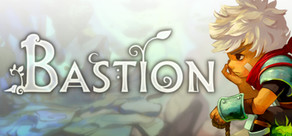
\includegraphics[scale=0.5]{img/cp07/img0702.png}

(fuente: http :// store . steampowered . com / app /107100 )
Es un Hack and slash (Hack and slash (literalmente "corta y
raja") es un género o estilo de videojuegos basados en los
combates) muy llamativo a primera vista por sus excelentes
gráficas en 1080, más de 10 armas mejorables únicas para usar,
un modo “Partida Nueva Plus” que se desbloquea al completar la
historia principal, cuenta con un narrador de voz dinámico que
acompaña a lo largo de todo el juego y se acoge a las decisiones
del jugador.

El juego tiene lugar en las postrimerías de la Calamidad, una
catástrofe que de repente se fracturó la ciudad de Caelondia ,
así como los alrededores del mundo del juego en muchos
pedazos flotantes, alterando su ecología y la reducción de la
mayor parte de su gente a cenizas. Los jugadores toman el
control de Kid, un protagonista silencioso que despierta en una
de las pocas piezas que quedan del viejo mundo y pone en
marcha para el titular Bastion, donde se suponía que todo el
mundo para ir en tiempos difíciles.

Esta disponible en Steam store y es jugable en una gran
variedad de plataformas:

\begin{itemize}
\item Microsoft Windows
\item Mac OS X
\item Xbox 360 (XBLA)
\item iOS
\item Google Chrome
\item Linux
\item OnLive
\end{itemize}

\subsection*{PLANESHIFT}
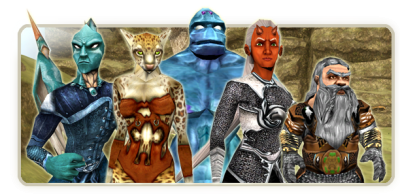
\includegraphics[scale=0.5]{img/cp07/img0703.png}

(fuente http :// www . planeshift . it /)
PlaneShift es un juego de rol inmerso en un mundo virtual de
fantasía en 3D, completamente hecho y mantenido por
voluntarios, se puede explorar el mundo virtual, interactuar con
otros jugadores o con criaturas controladas por el servidor,
luchar contra monstruos, lanzar hechizos, resolver misiones y
rompecabezas, mejorar tu personaje, obtener objetos mágicos,
posee diez tipos de razas diferentes cada una con caracteristicas
unicas, sistema original de magia con seis caminos de magia
diferentes, muchas ciudades y espacios libres para explorar, un
gran número de misiones para poner a prueba tu ingenio y
habilidad.

Gráficos 3D y sonidos para una experiencia de inmersión, se
ejecuta en todas las plataformas: Windows (Vista, XP, 2000),
Linux (x86 y amd64) y MacOSX, OpenGL con capacidad de
gráficos avanzados a través del motor Crystal Space 3D,
fácil interacción con otros jugadores a través de mensajes y el
chat y mucho mas.

PlaneShift es gratuita para todos los jugadores, utilizan dos
licencias, todo el código fuente del motor es de código abierto y
bajo licencia GPL. Esto significa que se puede reutilizar en otros
proyectos. Todos los demás activos son propiedad y derechos de
autor de Atomic Blue Corporation y no se permite su
reutilización.

\subsection*{FROZEN SYNAPSE}
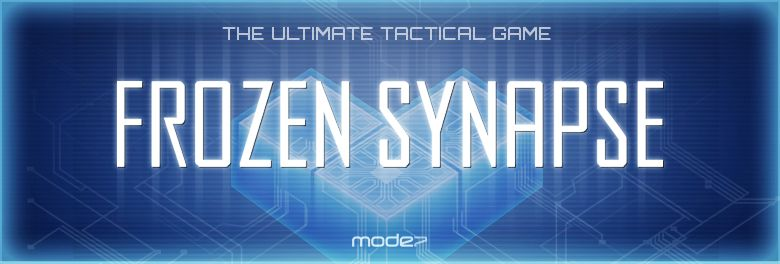
\includegraphics[scale=0.5]{img/cp07/img0704.png}
(fuente: http :// store . steampowered . com / app /98200/ )

Frozen Synapse es un juego de simulación de combate táctico,
en donde cada jugador controla un pequeño grupo de soldados
que se movilizan en un escenario que se genera de manera
pseudo-aleatoria asi como la posicion inicial de estos.

El objetivos de la mayoría de las misiones en modo de un solo
jugador es eliminar a el otro equipo, pero también cuenta con
tipos de misiones como proteccion de rehenes y escolta. En el
desarrollo de una partida multijugador se encuentran tipos de
juego protección del área, deathmatch al último hombre en pie y
extracción de rehenes.

Frozen Synapse esta disponible para Windows, OS X, Linux, iOS
y Android, actualmente disponible en la Steam Store para su
compra y uso en las plataformas Windows, Os X y Linux.


\subsection*{BRAID}

\includegraphics[scale=0.5]{img/cp07/img0705.png}

(Fuente http :// braid - game . com / )

Braid es un juego de plataformas y lógica, presentado con estilo
pictórico, donde es posible manipular el flujo del tiempo de
maneras inusuales y extrañas. Es protagonizado por Tim, un
hombre que esta en busca de su princesa, aunque no está muy
clara la relación de Tim con la princesa, la única parte que es
concreta es que él ha cometido algún tipo de error que espera
enmendar o borrar. Mientras el juego avanza a través de sus seis
mundos, un texto al principio de cada mundo nos revela mas
sobre la aventura de Tim en busqueda de su princesa.

Actualmente esta disponible para las plataformas GNU/Linux,
Mac Os X,Microsoft Windows, PSN,Xbox Live Arcade. Y es
posible acceder a él desde páginas como Steam, GamersGate y
Impulse bajo un costo de descarga.

